\newpage
\chapter{METODE PENELITIAN} \label{Bab III}

\section{Alur Penelitian} \label{III.Alur}
Keseluruhan proses penelitian dalam tugas akhir ini dirancang secara sistematis dan dituangkan ke dalam sebuah alur penelitian. Alur tersebut selanjutnya diilustrasikan melalui diagram alir yang disajikan pada Gambar \ref{fig:3.alur}. \par

\begin{figure}[H] % Kalau menggunakan H, posisi gambar akan tepat dibawah teks
    \centering
    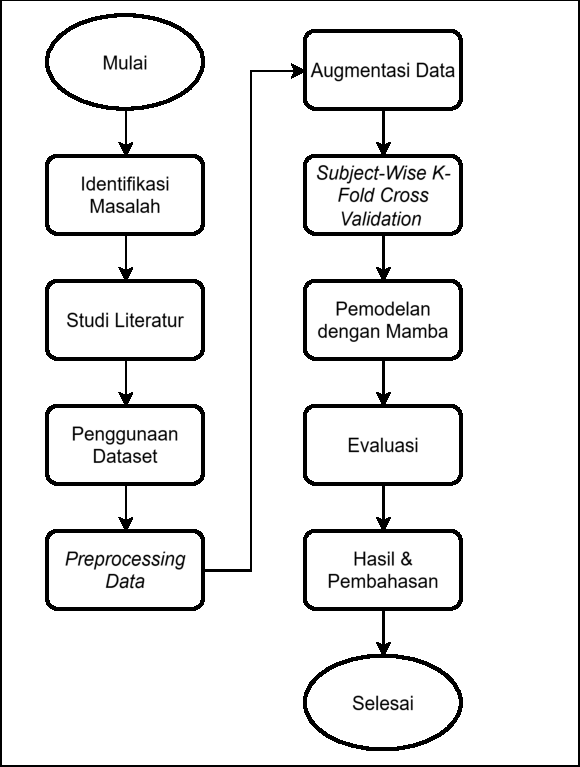
\includegraphics[width=0.6\textwidth]{figure/alur-penelitian.pdf}
    \caption{Alur Penelitian}
    \label{fig:3.alur}
\end{figure}

\section{Penjabaran Langkah Penelitian} \label{III.Jabar Alur}
Untuk memberikan pemahaman yang jelas mengenai metode yang digunakan, langkah-langkah dalam penelitian ini akan dijabarkan secara lebih terperinci. \par

\subsection{Identifikasi Masalah} \label{III.Langkah 1}
Tahap pertama dalam alur penelitian ini adalah identifikasi masalah, yang dilakukan untuk memetakan konteks dan urgensi dari penelitian. Proses ini diawali dengan analisis terhadap permasalahan di dunia nyata, yaitu tingginya risiko keselamatan yang disebabkan oleh kantuk saat berkendara. Analisis ini divalidasi dengan meninjau data statistik kecelakaan, seperti laporan BPS, serta studi pendukung yang mengonfirmasi bahwa pengemudi cenderung gagal menilai tingkat kantuk mereka secara objektif. \par

Setelah urgensi masalah teridentifikasi, proses dilanjutkan dengan menganalisis solusi sistem deteksi kantuk yang ada saat ini. Hasil analisis menemukan bahwa sebagian besar sistem komersial, seperti yang berbasis kamera, memiliki kelemahan fundamental, yaitu bersifat reaktif. Sistem tersebut baru memberikan peringatan setelah tanda-tanda fisik kantuk termanifestasi. Identifikasi kelemahan sistem reaktif ini menegaskan kebutuhan akan pendekatan yang lebih proaktif, sehingga penelitian ini difokuskan pada penggunaan sinyal fisiologis (EEG dan EOG) sebagai domain utama yang akan dieksplorasi. \par

\subsection{Studi Literatur} \label{III.Langkah 2}
Setelah masalah utama teridentifikasi, langkah selanjutnya dalam alur penelitian adalah melakukan studi literatur secara sistematis. Proses ini bertujuan untuk memvalidasi \textit{research gap} yang telah diidentifikasi pada Bab 1, mengumpulkan landasan teori yang relevan, serta memetakan metode \textit{state-of-the-art} (SOTA) yang akan digunakan sebagai pembanding dalam penelitian ini. \par

Studi literatur difokuskan pada tiga area utama. Pertama, meninjau arsitektur \textit{State Space Model} (SSM) dan Mamba, serta studi-studi terbaru yang menerapkannya pada sinyal EEG seperti klasifikasi tahap tidur. Kedua, mengidentifikasi metode SOTA yang ada saat ini khusus pada dataset DROZY, seperti model multimodal dari Cao et al. \cite{Cao2025Optimized}, untuk menetapkan \textit{benchmark} performa. Ketiga, studi ini secara khusus memvalidasi kesenjangan metodologis yang ditemukan di Bab 1, yaitu belum ditemukannya penerapan Mamba pada DROZY. \par

\subsection{Penggunaan Dataset} \label{III.Langkah3}
Penelitian ini menggunakan dataset publik "The ULg Multimodality Drowsiness Database" (DROZY). Dataset ini dirancang khusus untuk penelitian pemantauan kantuk dan berisi rekaman dari 14 subjek sehat (3 pria, 11 wanita). Proses pengumpulan data dilakukan dalam lingkungan laboratorium terkontrol di mana setiap subjek menjalani tiga sesi \textit{Psychomotor Vigilance Test} (PVT) berdurasi kurang lebih 10 menit. Sesi-sesi ini dilakukan dalam kondisi kekurangan tidur yang semakin meningkat, dengan total durasi kekurangan tidur mencapai 28 hingga 30 jam, untuk menginduksi kantuk secara alami. 

Sesuai dengan batasan masalah penelitian, data utama yang digunakan terdiri dari label kantuk subjektif serta sinyal fisiologis (EEG \& EOG) yang diekstrak dari rekaman \textit{Polysomnography} (PSG). Sinyal PSG dalam dataset ini direkam pada frekuensi 512 Hz dan mencakup 5 channel EEG (Fz, Cz, Pz, C3, C4) serta 2 channel EOG (vertikal dan horizontal). Sebagai \textit{ground truth} untuk melatih model, penelitian ini menggunakan Karolinska Sleepiness Scale (KSS), sebuah laporan subjektif 9-level (1=Sangat Segar, 9=Sangat Mengantuk) yang dicatat oleh subjek di awal setiap sesi PVT. Meskipun idealnya terdapat 42 rekaman (14 subjek $\times$ 3 sesi), beberapa data hilang dan satu sesi tidak dilakukan (7-1) akibat insiden teknis. Oleh karena itu, total bahan penelitian yang digunakan dalam penelitian ini adalah 36 set data (file .edf) \cite{Massoz2016}.

Terdapat 9 level pada skor KSS asli. Sejalan dengan pendekatan pada studi terbaru yang juga menggunakan dataset DROZY, tujuan utama dalam implementasi sistem adalah mendeteksi status mengantuk secara tegas, sehingga tidak diperlukan pembedaan yang terlalu spesifik pada tingkat kewaspadaan menengah \cite{zayed2025novel}. Berdasarkan rasionalisasi tersebut, pemrosesan label KSS pada penelitian ini dilakukan dalam dua skenario utama untuk mengakomodasi studi perbandingan:
\begin{enumerate}
    \item Skenario Klasifikasi (\textit{Train Baseline}): Untuk menyederhanakan tingkat kewaspadaan menengah menjadi keputusan akhir yang tegas, label skor KSS aktual dikelompokkan secara langsung menjadi klasifikasi biner (2 kelas) untuk pelatihan model \textit{baseline} klasifikasi \cite{zayed2025novel}. Pengelompokan dasar ini menggunakan batas kategori KSS 5, di mana kondisi \textit{Alert} secara mutlak didefinisikan untuk skor KSS diskrit 1-5, dan kondisi \textit{Drowsy} untuk skor KSS 6-9.

    \item Skenario Regresi (\textit{Train} \& Inferensi): Nilai KSS asli (1-9) dinormalisasi menjadi rentang kontinu $[0, 1]$ dengan cara membaginya menggunakan nilai maksimum KSS (9.0). Transformasi target ke rentang [0, 1] ini merupakan praktik esensial pada pemodelan regresi berbasis jaringan saraf untuk mencegah munculnya gradien kesalahan (\textit{exploding gradients}) yang ekstrem, sehingga algoritma optimasi dapat mencapai konvergensi dengan lebih cepat dan stabil. Pada tahap inferensi, setelah nilai prediksi dikembalikan ke skala asli (1-9), pemetaan ke kelas biner tidak menggunakan ambang batas bilangan bulat. Pemetaan dilakukan menggunakan nilai tengah sebesar 5.5. Keputusan ini diambil untuk mengakomodasi pembulatan matematis secara adil, di mana nilai prediksi $\le 5.5$ akan dikategorikan sebagai \textit{Alert} (mewakili rentang KSS 1-5), dan nilai $> 5.5$ dikategorikan sebagai \textit{Drowsy} (mewakili rentang KSS 6-9).
\end{enumerate}

\subsection{\textit{Subject Wise K-Fold Cross Validation}} \label{III.Langkah4}

Setelah tahap \textit{preprocessing}, validasi model dilakukan menggunakan \textit{subject-wise K-Fold Cross-Validation} dengan nilai $k = 5$. Pada skema ini, pembagian data dilakukan berdasarkan subjek, sehingga seluruh sampel dari satu subjek hanya muncul pada satu fold yang sama. Pada setiap iterasi, satu fold digunakan sebagai data uji dan $k-1$ fold lainnya sebagai data latih secara bergiliran. Pendekatan ini digunakan untuk mencegah kebocoran data antar subjek serta mengevaluasi kemampuan generalisasi model terhadap subjek yang belum pernah dilihat sebelumnya.

\subsection{\textit{Preprocessing} Data} \label{III.Langkah5}

Tahap prapemrosesan data bertujuan untuk mengubah data sinyal PSG mentah menjadi format sekuensial yang terstruktur dan siap digunakan oleh model Mamba. Proses prapemrosesan ini terdiri dari dua langkah utama, di mana langkah pertama adalah segmentasi sinyal menggunakan teknik \textit{sliding window}. Sinyal mentah 7 kanal (5 EEG: Fz, Cz, C3, C4, Pz, dan 2 EOG: EOG-V, EOG-H) yang direkam secara kontinu pada frekuensi 512 Hz dipotong dengan jendela pengamatan (\textit{window size}) berdurasi 30 detik. Pergeseran antar-jendela (\textit{stride}) ditetapkan selama 10 detik, sehingga secara otomatis menghasilkan area tumpang tindih (\textit{overlap}) sebesar 20 detik (sekitar 66\%) antar-segmen yang berdekatan. Mengacu pada frekuensi \textit{sampling} tersebut, setiap segmen 30 detik akan menghasilkan tensor berukuran $[7 \times 15.360]$ titik data yang diperlakukan sebagai satu sampel data individual. Pemilihan durasi 30 detik ini didasarkan pada metodologi yang digunakan oleh Zhao et al. (2024), yang merupakan penelitian \textit{state-of-the-art} untuk implementasi arsitektur Mamba pada kasus klasifikasi tingkat kantuk. Dalam studi tersebut, jendela waktu 30 detik dipilih karena merepresentasikan durasi standar satu \textit{epoch} sesuai pedoman klinis AASM \textit{(American Academy of Sleep Medicine)} untuk analisis tahapan tidur. Hal ini sangat penting karena memungkinkan model untuk menangkap dependensi temporal jangka panjang serta transisi bertahap antar-fase kesadaran yang sangat krusial \cite{Zhou2024Sleep}.

Selain tahapan segmentasi, dilakukan juga proses normalisasi sinyal. Berbeda dengan pendekatan standar yang umumnya melakukan normalisasi secara global pada setiap saluran (\textit{channel}) melintasi seluruh data, penelitian ini menerapkan teknik normalisasi berbasis subjek (\textit{subject-specific normalization}). Sinyal fisiologis seperti EEG dan EOG diketahui memiliki variabilitas antar-subjek (\textit{inter-subject variability}) yang tinggi, di mana amplitudo dan karakteristik dasar gelombang otak dapat berbeda secara signifikan antar individu, bahkan pada tingkat kewaspadaan yang sama. 

Oleh karena itu, normalisasi \textit{Z-score} diaplikasikan secara terpisah untuk setiap individu. Proses ini dilakukan dengan menghitung nilai rata-rata dan simpangan baku secara spesifik dari keseluruhan data rekaman milik satu subjek tertentu. Nilai amplitudo sinyal dari subjek tersebut kemudian dikurangi dengan rata-ratanya sendiri dan dibagi dengan simpangan bakunya masing-masing. Alur komputasi ini diulangi untuk setiap subjek yang ada di dalam dataset. Melalui pendekatan ini, data sinyal dari setiap pengemudi akan memiliki skala yang seragam, sehingga model Mamba dapat lebih fokus dalam mengekstraksi pola penurunan kewaspadaan yang relatif dari masing-masing individu tanpa terdistorsi oleh perbedaan karakteristik bawaan antar subjek.

\subsection{Augmentasi Data} \label{III.Langkah6}
Proses augmentasi pada penelitian ini dilakukan secara dinamis (\textit{on-the-fly}) pada setiap \textit{epoch} pelatihan. Terdapat dua teknik transformasi yang diaplikasikan secara independen, di mana masing-masing teknik memiliki probabilitas sebesar 50\% untuk diterapkan pada setiap segmen sampel sinyal. Penggunaan parameter yang kecil (\textit{mild augmentation}) ini dirancang secara spesifik untuk sinyal biologis, guna memastikan bahwa penambahan variasi tidak merusak informasi penting yang terkandung di dalamnya. Kedua teknik tersebut adalah:
\begin{enumerate}
    \item \textit{Gaussian Noise}: Penyuntikan derau acak berdistribusi normal ke dalam sinyal untuk menyimulasikan gangguan pada sensor maupun variasi biologis minor. Parameter derau yang ditambahkan memiliki standar deviasi (\textit{STD}) sebesar 0.01.
    \item \textit{Amplitude Scaling}: Pengubahan skala amplitudo sinyal secara acak untuk menyimulasikan variabilitas kekuatan sinyal antar-subjek maupun antar-sesi perekaman. Faktor skala ditarik secara acak dari rentang 0.9 hingga 1.1.
\end{enumerate}

Melalui penerapan probabilistik dari kedua teknik ini, model Mamba dilatih untuk mengekstrak representasi fitur temporal yang lebih tangguh (\textit{robust}) tanpa kehilangan pola fundamental dari sinyal kantuk itu sendiri.

\subsection{Pemodelan dengan Mamba} \label{III.Langkah7}

Sesuai dengan alur penelitian, setelah data mentah disiapkan melalui tahap \textit{preprocessing}, langkah selanjutnya adalah tahap pemodelan dengan Mamba. Tahap ini merupakan inti dari eksperimen penelitian, di mana model \textit{deep learning} yang diusulkan akan dibangun, dilatih, dan divalidasi. Pada bagian ini, akan dijelaskan proses penggunaan arsitektur Mamba untuk memproses sekuens sinyal EEG dan EOG yang telah disegmentasi. Tujuan utama dari model ini adalah untuk mempelajari pola-pola temporal kompleks di dalam sinyal tersebut yang berkorelasi dengan 2 kategori tingkat kantuk yang didasari dari skor KSS.

\subsection{Evaluasi} \label{III.Langkah8}
Evaluasi kinerja model dalam penelitian ini dilakukan secara menyeluruh mencakup aspek ketepatan prediksi dan efisiensi komputasi. Untuk mengukur performa prediksi pada tahap pelatihan regresi, digunakan metrik \textit{Mean Absolute Error} (MAE). Sementara itu, pada tugas klasifikasi biner di tahap inferensi akhir, digunakan metrik Akurasi, Presisi, \textit{Recall}, dan \textit{F1-Score}. Akurasi mengukur persentase total prediksi yang benar, Presisi menghitung proporsi prediksi positif yang relevan, sedangkan \textit{Recall} mengukur kemampuan model mendeteksi seluruh sampel positif (yaitu kelas \textit{Drowsy}). \textit{F1-Score} kemudian dihitung sebagai rata-rata harmonik antara Presisi dan \textit{Recall}. Di samping itu, efisiensi komputasi model dievaluasi melalui pengukuran GFLOPs untuk mengestimasi kompleksitas operasi dan jumlah parameter untuk mengetahui kapasitas spasial model. Terakhir, \textit{Confusion Matrix} digunakan untuk memvisualisasikan hasil klasifikasi biner agar distribusi kesalahan antara kelas \textit{Alert} dan \textit{Drowsy} dapat dianalisis secara detail.

\section{Lingkungan Pengembangan Tugas Akhir} \label{III.Lingkungan Pengembangan}
Pelaksanaan penelitian ini membutuhkan lingkungan pengembangan yang memadai, baik dari sisi komputasi fisik maupun perangkat lunak, guna mendukung kelancaran proses pra-pemrosesan data sinyal fisiologis hingga pelatihan arsitektur \textit{deep learning} yang kompleks. Lingkungan pengembangan ini dibagi menjadi dua kategori utama, yaitu perangkat keras dan perangkat lunak.

\subsection{Perangkat Keras (\textit{Hardware})}
Perangkat keras utama yang digunakan dalam penelitian ini adalah satu unit laptop Asus Vivobook M415DA yang berfungsi sebagai stasiun kerja utama untuk penulisan kode, analisis data tahap awal, serta manajemen repositori proyek. Laptop yang digunakan beroperasi dengan sistem operasi Windows 11, serta ditenagai oleh prosesor AMD Ryzen 3-3250U, memori RAM sebesar 8 GB, dan media penyimpanan SSD berkapasitas 512 GB. 

Meskipun arsitektur Mamba dirancang dengan tingkat efisiensi komputasi yang tinggi, implementasi dan kompilasi library intinya saat ini sangat dioptimalkan dan lebih stabil untuk berjalan pada ekosistem sistem operasi berbasis Linux. Mengingat perangkat keras lokal beroperasi menggunakan Windows 11, laptop ini utamanya berperan sebagai antarmuka untuk pengembangan skrip awal. Untuk menghindari kendala kompatibilitas sistem operasi dan mempermudah proses kompilasi pustaka CUDA, eksekusi pelatihan model secara penuh dilakukan melalui layanan \textit{cloud computing} yang telah menyediakan lingkungan Linux secara \textit{native} beserta dukungan unit pemrosesan grafis (GPU).

\subsection{Perangkat Lunak (\textit{Software})}
Selain perangkat keras, penelitian ini juga sangat bergantung pada susunan perangkat lunak (\textit{software stack}) yang saling terintegrasi. Beberapa perangkat lunak utama yang digunakan meliputi:
\begin{enumerate}
    \item Bahasa Pemrograman Python: Digunakan sebagai bahasa pemrograman utama karena kapabilitasnya yang sangat luas dan dukungan ekosistem pustaka (\textit{library}) yang matang untuk keperluan \textit{machine learning} dan pemrosesan sinyal.
    \item PyTorch: Berfungsi sebagai \textit{framework} \textit{deep learning} utama untuk membangun, melatih, dan mengevaluasi arsitektur Mamba. PyTorch dipilih karena fleksibilitasnya dalam komputasi tensor dinamis berbasis GPU.
    \item Google Colab: Digunakan sebagai platform komputasi awan berbasis \textit{Jupyter Notebook} untuk mengeksekusi kode secara interaktif dan mendapatkan akses ke sumber daya GPU secara efisien tanpa terkendala spesifikasi perangkat keras lokal.
    \item Visual Studio Code (VS Code): Berfungsi sebagai \textit{Integrated Development Environment} (IDE) lokal untuk menulis, merapikan, dan menguji skrip pemrograman.
    \item Git dan GitHub: Digunakan sebagai (\textit{version control system}) untuk merekam jejak perubahan kode, serta menyimpan cadangan repositori proyek secara aman.
    \item Weights \& Biases: Digunakan sebagai pustaka pendukung untuk memantau, mencatat metrik evaluasi (seperti MAE dan \textit{Loss}), serta mengelola parameter selama proses eksperimen dan pelatihan model berlangsung.
\end{enumerate}

\section{Metode Pengembangan} \label{III.Metode}

\begin{figure}[H]
    \centering
    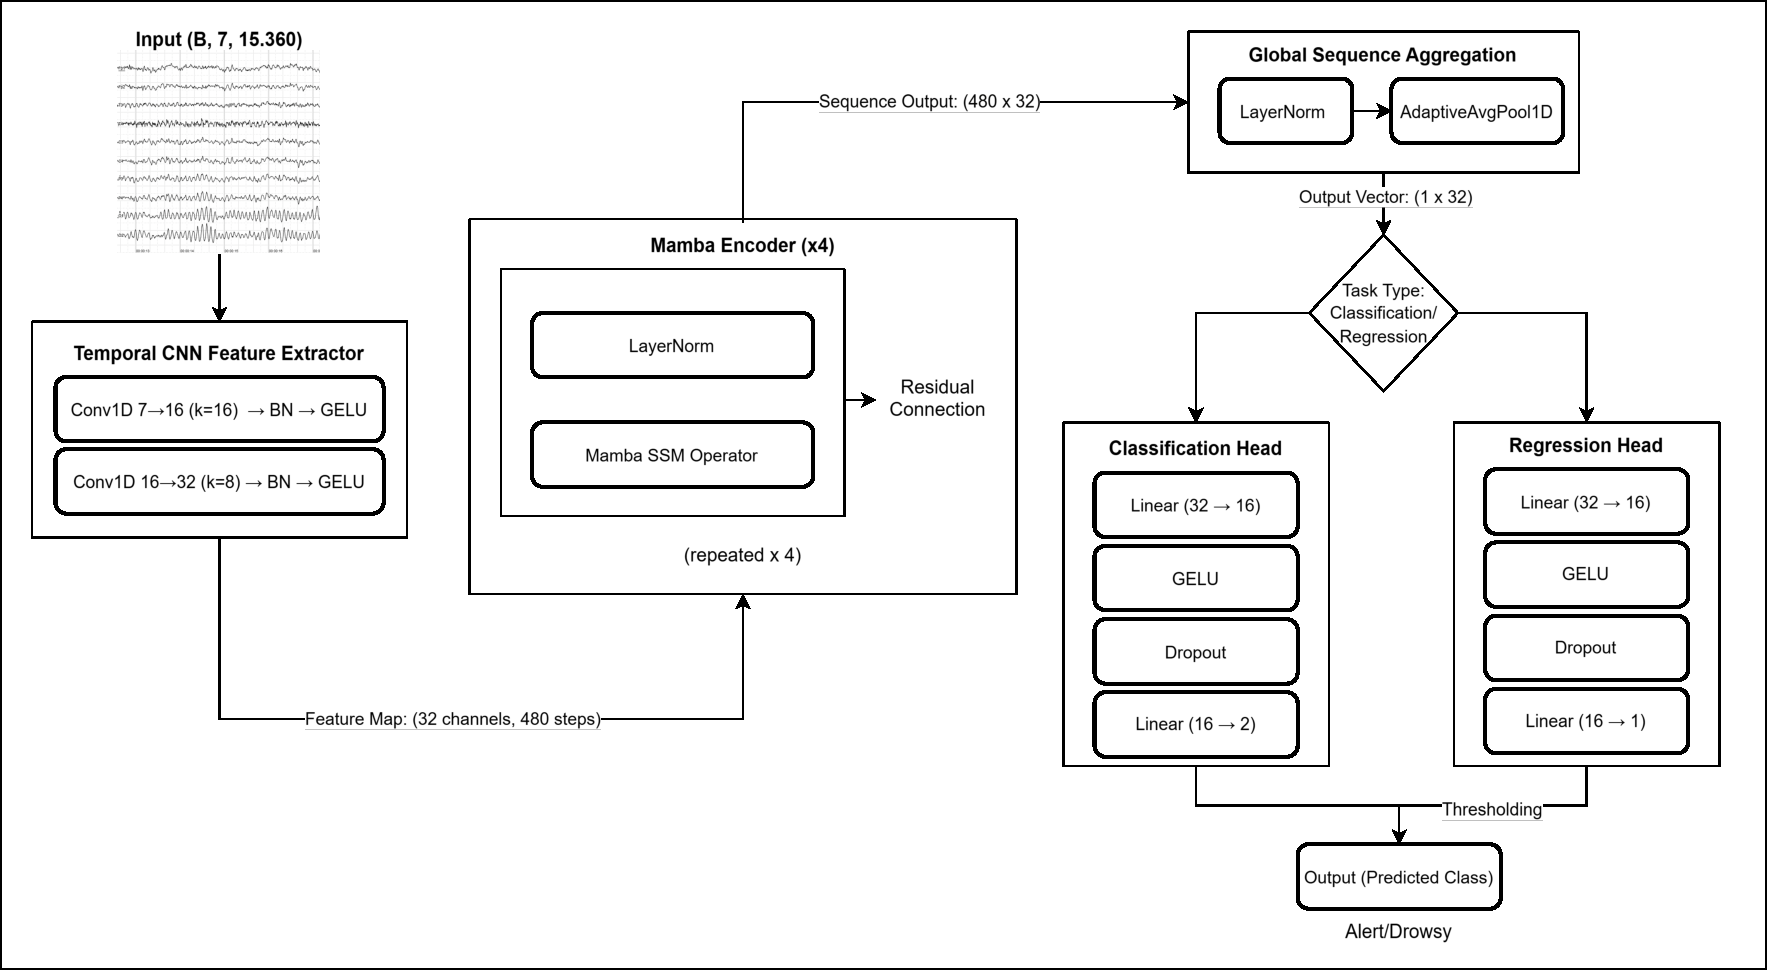
\includegraphics[width=1\textwidth]{figure/model-alur.pdf}
    \caption{Pemodelan dengan Mamba}
    \label{fig:3.mamba-model}
\end{figure}

Arsitektur pemodelan, sebagaimana diilustrasikan pada Gambar \ref{fig:3.mamba-model}, dirancang untuk memproses segmen data yang telah dipersiapkan pada tahap \textit{preprocessing}. Model menerima masukan data 30 detik dengan dimensi \texttt{Input (B, 7, 15.360)}, yang merepresentasikan 7 \textit{channel} (5 EEG + 2 EOG). Masukan ini pertama kali diproses oleh \textit{Temporal CNN Feature Extractor} yang terdiri dari dua lapisan \textit{Conv1D} dengan konfigurasi filter $7 \rightarrow 16$ ($k=16$) dan $16 \rightarrow 32$ ($k=8$), yang masing-masing diikuti oleh \textit{Batch Normalization} (BN) dan fungsi aktivasi GELU. Proses ini menghasilkan \textit{Feature Map} dengan dimensi (32 \textit{channels}, 480 \textit{steps}) yang mereduksi panjang sekuens namun memperkaya representasi fitur temporal lokal.

Inti dari arsitektur ini adalah \textit{Mamba Encoder} (\textit{x4 block}), yang terdiri dari 4 blok Mamba yang ditumpuk secara berulang. Setiap blok terdiri dari \textit{LayerNorm} dan \textit{Mamba SSM Operator} dengan tambahan \textit{Residual Connection} untuk menjaga stabilitas aliran gradien. Pemilihan arsitektur \textit{State Space Model} (SSM) ini didasarkan pada efisiensi komputasi linear ($O(n)$) yang memungkinkan model secara selektif menentukan informasi temporal jangka panjang pada sinyal EEG dan EOG yang harus dipertahankan atau diabaikan melalui mekanisme \textit{selective state spaces} \cite{Gu2023}.

Setelah melalui blok Mamba, \textit{Sequence Output} berdimensi ($480 \times 32$) diteruskan ke tahap \textit{Global Sequence Aggregation}. Pada tahap ini, data diproses melalui \textit{LayerNorm} dan \textit{AdaptiveAvgPool1D} untuk menghasilkan \textit{Output Vector} tunggal berdimensi ($1 \times 32$). Bergantung pada jenis tugas, vektor ini akan diteruskan ke salah satu dari dua \textit{head} yang berbeda. Jika yang sedang dikerjakan adalah tugas klasifikasi, maka vektor akan diteruskan ke \textit{Classification Head} yang terdiri dari lapisan \textit{Linear} ($32 \rightarrow 16$), GELU, \textit{Dropout}, dan \textit{Linear} $16 (\rightarrow 2$) untuk menghasilkan probabilitas kelas secara langsung. Sedangkan jika yang sedang dikerjakan adalah tugas regresi, maka vektor akan diteruskan ke \textit{Regression Head} yang terdiri dari lapisan \textit{Lienar} ($32 \rightarrow 16$), GELU, \textit{Dropout}, dan \textit{Linear} ($16 \rightarrow 1$) untuk menghasilkan skor kontinu.

Khusus untuk pendekatan regresi, nilai keluaran kontinu tersebut kemudian diproses melalui tahap \textit{Thresholding} untuk menghasilkan keputusan akhir berupa \textit{Output (Predicted Class)}. Seluruh alur ini dievaluasi menggunakan skema \textit{subject-wise} 5-\textit{Fold Cross-Validation} untuk memastikan model mampu melakukan generalisasi terhadap kondisi \textit{Alert} atau \textit{Drowsy} dari subjek yang belum pernah dilihat sebelumnya.

\section{Ilustrasi Perhitungan}
Untuk memberikan pemahaman yang lebih jelas tentang proses perhitungan metrik evaluasi, bagian ini menyajikan ilustrasi perhitungan \textit{end-to-end} menggunakan sampel data simulasi.

Berikut ini adalah contoh \textit{confusion matrix} yang digunakan sebagai contoh ilustrasi perhitungan evaluasi.

\begin{figure}[H]
    \centering
    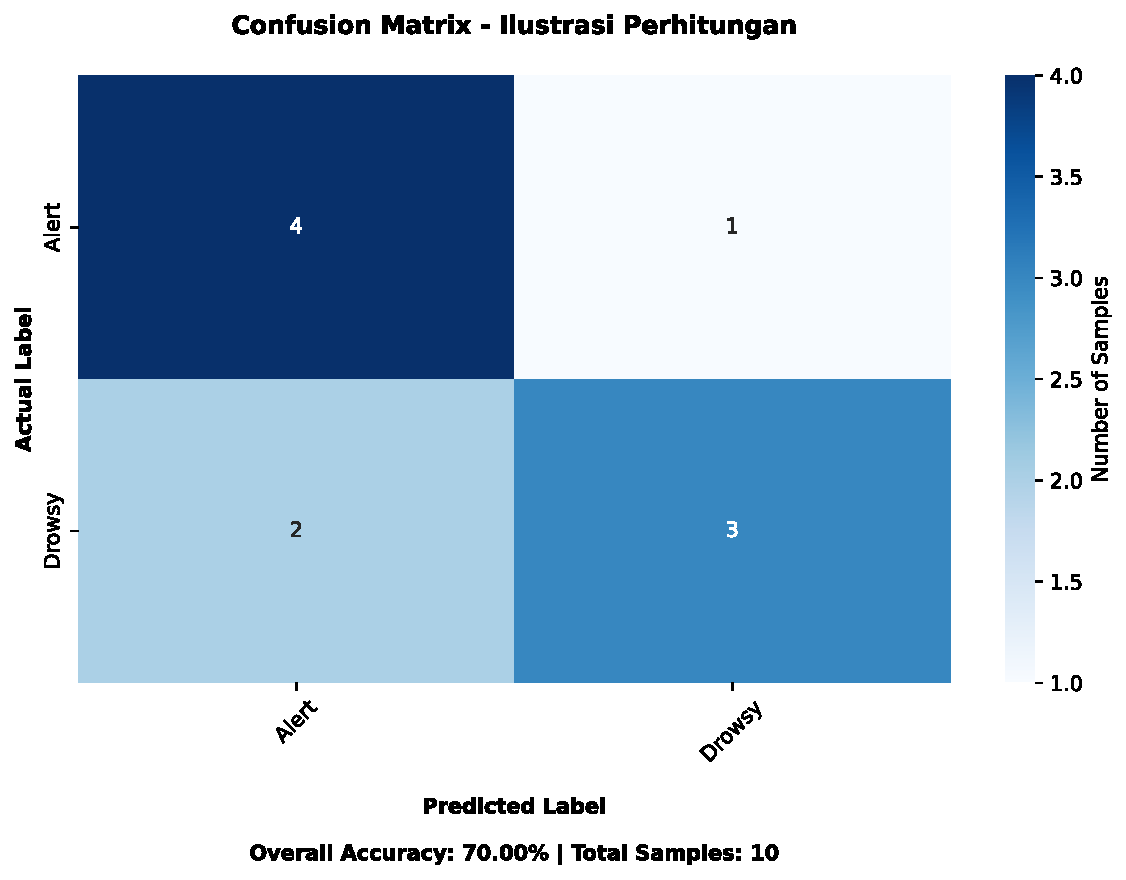
\includegraphics[width=1\textwidth]{figure/conf2x2.pdf}
    \caption{Ilustrasi Confusion Matrix}
    \label{fig:3.ill-conf}
\end{figure}

\textit{Confusion Matrix} yang disajikan pada Gambar \ref{fig:3.ill-conf} memvisualisasikan kinerja klasifikasi model untuk dua tingkat kantuk: \textit{Alert} dan \textit{Drowsy}. Dalam matriks ini, label aktual disusun sebagai baris sementara label prediksi ditempatkan sebagai kolom, di mana setiap sel merepresentasikan jumlah sampel untuk kombinasi klasifikasi tertentu. Sebagai ilustrasi, angka 4 pada pertemuan baris dan kolom \textit{Alert} (diagonal utama) menunjukkan bahwa model berhasil memprediksi 4 sampel \textit{Alert} dengan tepat. Distribusi nilai dalam keseluruhan matriks ini menjadi landasan fundamental untuk perhitungan metrik evaluasi kuantitatif, meliputi \textit{accuracy, precision, recall}, dan \textit{f1-score}.

\subsection{\textit{Precision}}
Precision untuk mengukur ketepatan prediksi setiap kelas. Berdasarkan rumus 2.7, \textit{precision} dihitung pada masing-masing kelas dengan rincian sebagai berikut.

\[
\text{Precision}_{Alert} = \frac{4}{4 + 2} = \frac{4}{6} \approx 0.67
\]
\vspace{1em}

\[
\text{Precision}_{Drowsy} = \frac{3}{3 + 1} = \frac{3}{4} = 0.75
\]

\subsection{\textit{Recall}}
Recall mengukur kemampuan model mengenali sampel yang benar-benar berasal dari suatu kelas. Berdasarkan rumus 2.8, \textit{recall} dihitung pada masing-masing kelas dengan rincian sebagai berikut:

\[
\text{Recall}_{Alert} = \frac{4}{4 + 1} = \frac{4}{5} = 0.80
\]
\vspace{1em}

\[
\text{Recall}_{Drowsy} = \frac{3}{3 + 2} = \frac{3}{5} = 0.60
\]

\subsection{\textit{F1-Score}}
F1-score merupakan rata-rata harmonik antara \textit{precision} dan \textit{recall}. Berdasarkan rumus 2.9, \textit{f1-score} dihitung pada masing-masing kelas dengan rincian sebagai berikut:

\[
\text{F1}_{Alert} = 2 \times \frac{(0.67)(0.80)}{0.67 + 0.80} = \frac{1.072}{1.47} \approx 0.73
\]
\vspace{1em}

\[
\text{F1}_{Drowsy} = 2 \times \frac{(0.75)(0.60)}{0.75 + 0.60} = \frac{0.90}{1.35} \approx 0.67
\]

\subsection{\textit{Accuracy}}
Accuracy menggambarkan proporsi prediksi benar dibandingkan seluruh sampel. Berdasarkan rumus 2.6, \textit{accuracy} dihitung dengan rincian sebagai berikut:

\[
\text{Accuracy} = \frac{4 + 3}{10} = \frac{7}{10} = 0.70
\]

\section{Rancangan Pengujian}

Proses pengujian terhadap model yang telah dilatih dilakukan secara menyeluruh dengan mencakup dua aspek utama, yaitu kinerja klasifikasi dan efisiensi komputasi model. Kinerja klasifikasi dievaluasi berdasarkan \textit{confusion matrix} yang menjadi dasar perhitungan empat metrik evaluasi utama, yaitu \textit{accuracy}, \textit{precision}, \textit{recall}, dan \textit{F1-score}. 

Selain itu, untuk menilai efisiensi komputasi dari sisi arsitektural, evaluasi dilakukan menggunakan metrik jumlah parameter (\textit{parameter count}) dan \textit{Giga Floating Point Operations} (GFLOPs). Kedua metrik ini digunakan untuk merepresentasikan kompleksitas model secara perangkat-agnostik, sehingga memungkinkan perbandingan efisiensi komputasi yang lebih adil dan konsisten antar arsitektur.
